\documentclass{article}%
\usepackage[T1]{fontenc}%
\usepackage[utf8]{inputenc}%
\usepackage{lmodern}%
\usepackage{textcomp}%
\usepackage{lastpage}%
\usepackage{pgf}%
\usepackage{hyperref}%
\usepackage{pdflscape}%
\usepackage{float}%
\usepackage{listings}%
\usepackage{graphicx}%
\usepackage{ragged2e}%
\usepackage{listings}

%
\title{%
Semestrální projekt NI-PDP 2021/2022 \\
\large Paralelní algoritmus pro řešení problému nalezení bipartitního podgrafu s maximální váhou}%
\author{Martin Skalický}%
\date{\today}%
%
\begin{document}%
\normalsize%
\maketitle%
\section{Zadání}%
\label{sec:Zadn}%
Cílem této práce je implementace a analýza paralelního algoritmu pro řešení problému nalezení bipartitního podgrafu s maximální váhou. Nechť \textit{n} je přirozené číslo představující počet uzlů grafu \textit{G}, 50 > \textit{n} >= 10, dále \textit{k} je přirozené číslo představující průměrný stupeň uzlu grafu \textit{G}, \textit{n}/2 >= \textit{k} >= 3. Graf \textit{G(V,E)} je jednoduchý neorientovaný hranově ohodnocený souvislý graf o \textit{n} uzlech a průměrném stupni \textit{k}, váhy hran jsou z intervalu \textit{<80,120>}.

Graf \textit{G(V,E)} je \textbf{bipartitní}, pokud lze množinu uzlů V rozdělit na disjunktní podmnožiny \textit{U} a \textit{W} tak, že každá hrana v \textit{E} spojuje uzel z \textit{U} s uzlem z \textit{W}. Jinak řečeno, bipartitní graf lze uzlově obarvit 2 barvami 0 a 1. Úkolem je nalézt podmnožinu hran \textit{F} takovou, že podgraf \textit{G(V,F)} je souvislý a bipartitní a váha \textit{F} je \textbf{maximální} v rámci všech možných bipartitních souvislých podgrafů \textit{G} nad \textit{V}.

\subsection{Vstup algoritmu}
Soubor obsahující definici grafu. První řádek obsahuje číslo \textit{n} definující počet uzlů v grafu. Další řádky obsahují všechny cesty v grafu definované pomocí matice sousednosti o velikosti \textit{n} * \textit{n}, kde jednotlivé prvky odpovídají ohodnocení danné cesty.

\subsection{Výstup algoritmu}
Výpis všech bipartitních podgrafů s maximální váhou: výpis obou podmnožin \textit{U} a \textit{W} uzlů bipartitního souvislého podgrafu, výpis množiny jeho hran a výpis hodnoty součtu jejich vah.

%
\section{Popis sekvenčního algoritmu}%
\label{sec:Popissekvencni}%
\begin{itemize}
    \item Řešení existuje vždy, vždy lze v souvislém grafu \textit{G} zkonstruovat souvislý bipartitní podgraf nad \textit{V}, neboť lze vždy zkonstruovat kostru \textit{G}.
    \item Souvislých bipartitních podgrafů s maximální cennou může být více.
    \item Sekvenční algoritmus je typu \textit{BB-DFS} s hloubkou stavového stromu omezenou |E|.
    \item Pokud je graf \textit{G} bipartitní, pak triviálně F=E, jinak \textit{F} je podmnožinou \textit{E}.
    \item \textbf{Přípustný mezistav} tvoří každá podmnožina hran \textit{F} taková, že podgraf \textit{G(V,F)} je bipartitní.
    \item \textbf{Cena}, kterou maximalizujeme, je součet cen hran v \textit{F}.
    \item \textbf{Přípustný koncový stav} je tvořen takovou podmnožinou hran \textit{F}, do které už nelze žádnou další přidat, aniž by se porušila bipartitnost.
\end{itemize}%

Algoritmus dostane list barev uzlů \textit{nodes} (zatím neobarvené) a list všech hran grafu \textit{edges}. Nejprve je první uzel označen barvou 0 (pro eliminaci druhého stejného řešení s přehozenými barvami). Následně je spuštěný DFS algoritmus, který postupně zpracovává jednolivé hrany. Pro jednotlivé hrany nastávají následující 3 možnosti (ternární rekurzivní strom volání):
\begin{itemize}
    \item hrana je zařazena do \textit{F} a označena barvou 0, provede se test, zda toto obarvení je v souvladu s dosud vybudovaným bipartitním podrafem, pokud není, tak je proveden návrat
    \item hrana je zařazena do \textit{F} a označena barvou 1, provede se test, zda toto obarvení je v souvladu s dosud vybudovaným bipartitním podrafem, pokud není, tak je proveden návrat
    \item hrana není zařazena do \textit{F}
\end{itemize}

% Ořezávání
Pro zvýšení výkonosti algoritmu je využito průběžné ořezávání prohledávaného prostoru. V každém mezistavu je průběžně počítána cena hran zařazených do \textit{F}. Větev je předčasně ukončena pokud v daném mezistavu je zjištěno pomocí horního odhadu váhy zbývajícího bipartitiního podgrafu, že z něj nelze žádným způsobem vytvořit přípustný koncový stav \textit{(V,F)} s větší cenou \textit{F}, než dosud nalezené nejlepší řešení - horní odhad je vypočten jako součet cen zařazených hran do \textit{F} a cen zbývajících ještě nezpracovaných hran.

Po dosažení koncového stavu je proveden test souvislosti grafu \textit{G(V,F)}. Pokud je graf souvislý, tak je jeho cena porovnána s doposud nejlepším a pokud má stejnou cenu, tak je přidáno a pokud vyšší, tak nahradí doposud nejlepší řešení, jinak je řešení zamítnuto.


\section{Implementace}
Pro implementaci byl zvolen jazyk \textit{C++}, kvůli autorově oblibě vyšší abstrakce než nabízí jazyk C.

\subsection{Sekvenční algoritmus}
Cesta k souboru s definicí grafu je programu předána pomocí parametru. Po spuštění si program soubor načte a vytvoří si dočasnou reprezentaci matice sousednosti jako jednorozměrné pole. Následně je z této matice sousednosti vytvořen seznam všech hran grafu (dále jako \textit{edges}), kde každá hrana obsahuje svoji cenu a čísla vrcholů, které spojuje. Pro zvýšení účinosti ořezávání (dále bude upřesněno) je seznam hran seřazen sestupně dle ceny. Je vytvořen pomocný list (dále jako \textit{nodes}), jehož délka je rovna počtu uzlů a i-tý prvek obsahuje barvu i-tého uzlu. Na počátku jsou všechny uzly neobarvené. Před spuštěním samotného algoritmu je nejprve zkontrolováno zda graf není bipartitní, potom by byl sám řešením a nebylo by potřeba algoritmus spouštět. Pro kontrolu bipartitnosti, je nejprve vytvořen seznam všech sousedů pro každý uzel a následně se vezme první uzel a pomocí BFS algoritmu se projde celý graf a obarví se všechny dosažitelné vrcholi. Pokud bylo možné obarvit bipartitně všechny uzly, tak byl graf bipartitní a bylo nalezeno řešení. V opačném případě je spuštěn samotný DFS algoritmus pro nalezení řešení.

V každé větvi DFS je k dispozici množina dosud použitých hran \textit{F}, množina ještě nezpracovaných hran, aktuálně zpracovávaná hrana a obarvení jejích vrcholů. Na začátku je zkontrolováno zda součet cen množiny hran \textit{F} a ještě nezpracovaných hran. Pokud je nižší než dosud nejlepší nalezené řešení, tak je tato větev předčasně ukončena. Následně je provedena kontrola, zda při příslušném obarvení může být dosud nalezený podgraf bipartitní. Pokud není, tak je větev předčasně ukončena. Pokud již nejsou ke zpracování další hrany, tak je zkontrolováno zda \textit{G(V,F)} tvoří souvislý podgraf (předchozí kontrola bipartnitnosti zaručuje, že pokud je souvislý, tak je i bipartitní). Pokud je souvislý a jeho cena je rovna doposud nejlepšímu, tak je řešení přidáno do výsledku. Pokud je řešení lepší než doposud nejlepší, tak ho nahradí.

Pokud seznam nezpracovaných hran ještě není prázdný, tak je jedna hrana odebrána. Následně jsou spuštěny 3 rekurzivní DFS algoritmy se seznamem hran ke zpracování bez této odebrané, kterou:
\begin{itemize}
    \item Zařadí hranu do \textit{F} a označí obravení uzlů hrany barvami 0, 1.
    \item Zařadí hranu do \textit{F} a označí obravení uzlů hrany barvami 1, 0.
    \item Zachová původní množinu \textit{F} (vynechá hranu).
\end{itemize}%

Sběr nejlepších řešení jsem prvotně řešil tak, že návratová hodnota z větva byla množina všech nejlepších řešení dané větve, tyto výsledky z větvení byly zkombinovány a bylo vráceno toto řešení. Později jsem toto řešení upravil z důvodu výkonosti tak, že všechna nejlepší řešení (řešení s doposud nejvyšší cenou) obsahuje globální proměnná, do které je vloženo řešení ihned po jeho nalezení.


\subsection{OpenMP - tasl paralelismus}
Task paralelismus v OpenMP funguje tak, že je jedna společná množina, ze které si jednotlivá vlákna berou úkoly, pokud zrovna žádný nezpracovávají. Případně pokud vytvoří nový úkol, tak ho do dané množiny vloží. Implicitně není zaručeno pořadí zpracování úkolů.
Implementace vyžadovala drobný zásach do sekvenčního řešení přidáním příslušných OpenMP direktiv. Nejprve bylo potřeba zajistit, aby došlo ke spuštění DFS algoritmu pouze jednou pomocí ``omp single``.

\begin{lstlisting}[language=c++]
#pragma omp parallel default(shared)
{
    #pragma omp single
    findSolutions(Edge{}, NONE, nodes, edges, acc);
}
\end{lstlisting}

Prvním parametrem funkce algoritmu je aktuálně zpracovávaná hrana, druhý parametr je varianta obarvení uzlů hrany, třetí je list aktuálního obarvení uzlů, čtvrtým jsou nezpracované hrany a poslední obsahuje aktuálně sestavený podgraf a jeho cenu. Toto volání zajistilo prvotní spuštění algoritmu, který následně vytvoří 3 další úkoly pro vlákna (ternární rekurzivní strom volání). Ukázka jednoho větvení:
\begin{lstlisting}[language=c++]
#pragma omp task shared(bestWeight) 
    |> if (edges.data.size() > TASK_SIZE)
findSolutions(edge, RED, nodes, edges, acc);
\end{lstlisting}
Tímto došlo k vytváření jednotlivých úkolu, která si vlákna paralelně odebírají ke zpracování a generují nové. Poslední důležitou věcí bylo zajistit aktualizaci globálního nejlepšího řešení, protože při paralelním zápisu by docházelo k race condition. Toho bylo docílo pomocí využití OpenMP kritické sekce v rámci které došlo k porovnání cen aktuálně nejlepšího a nového a případné změně či přidání.

Větvení obsahuje podmínku, za které ještě má dojít k vytváření paralelních úkolů nebo dané vlákno má dokončit výpočet. Toto umožňuje snížit overhead, který nastává při generování paralelních úkolů a jejich rozdělování. Experimentálně jsem zkoušel nastavit různé velikosti TASK\_SIZE a 12 se ukázalo jako dobrý kompromis.

\subsection{OpenMP - datový paralelismus}
Datový paralelismus se ve své podstatě od task paralelismu moc neliší. Oba jsou založeny na tom, že je k dispocizi množina úkolů, které musejí vlákna zpracovat. Hlavní rozdíl spočívá v tom, že při datovém je již předem vygenerována celá množina úkolů a vlákna již provádějí pouze výpočet. Tatímco při táskovém paralelismu mohou vlákna přidávat nové úkoly do množiny. Je tedy důležité vytvořit dostatečně velké množství úkolů, protože kvůli průběžnému ořezávání se mohou úkoly diametrálně lišit ve výpočetní obtížnosti. Současně je ale potřeba brát v úvahu, že vyšší počet se bude generovat delší dobu a zabere větší množství paměti. Je tedy potřeba najít určitý kompromis.

Algoritmus pro prvotní gerování úkolů má vstupem cílový počet úkolů, které má vygenerovat a prvotní problém, který je reprezentován parametry, které odpovídají vstupním parametrům sekvenčního algoritmu. Výstupem je list úkolů, kde každý úkol je reprezentován parametry, které lze předat sekvenčnímu algoritmu pro řešení. Algoritmus prochází ternární rekurzivní strom volání, který vytváří sekvenční DFS algoritmus, pomocí BFS postupně po jednotlivých hladinách. Výsledkem jsou listy z procházeného stromu volání (o cílovém počtu), které se liší v hladínách maximálně o jedna - měli by teoreticy být podobně obtížné (teoreticky, protože ořezávání ovlivňuje obtížnost).

Nad takto vygenerovanými úkoly, je následně spuštěn OpenMP paralelní cyklus, který průběžně přiřazuje úkoly vláknům. Aktualizace nejlepšího řešení probíhá pomocí kritické sekce stejně jako v případě task paralelismu.
\begin{lstlisting}[language=c++]
#pragma omp parallel for schedule(dynamic)
for (int i = 0; i < q.size(); i++) {
    auto &partial = q[i];
    findSolutions(partial.edge, partial.variant,
        partial.nodes, partial.edges, partial.acc);
}
\end{lstlisting}

Počet generovaných úkolů jsem odhadl a experimentálně ověřil na několika větších instancích - sledoval jsem využití CPU v průběhu běhu algoritmu. Generuje se 70krát počet výpočetních vláken.

\subsection{MPI s OpenMP datovým paralelismem}
MPI je knihovna pro meziprocesorovou komunikaci s jejíž pomocí lze paralelismus škálovat na více výpočetních uzlů. Architektura paralelismu bude typu Master-Slave. Jeden proces bude Master, který vygeneruje příslušný počet problémů v závislosti na počtu procesů (stejně jako v případě datového paralelismu a závislosti na počtu vláken) a následně bude problémy k řešení rozesílat na ostatní procesy k samotnému výpočtu. Proces typu Slave bude čekat dokud neobdrží úkol od Masteru a začně problém řešit pomocí datového paralelismu (viz. předchozí bod). Rozhodl jsem se pro datový paralelismus oproti task paralelismu, protože nad testovacími daty se ukázal jako výkonější a časově stabilnější. Slave po ukončení výpočtu odešle nalezené řešení zpět na Master a opět čeká až dostane další problém k řešení. Master získává průběžně řešení všech problémů a z nich si udržuje taková, která dosáhla nejvyšší ceny.

Pro implementaci jsem využil knihovnu \textbf{boost} a její nadstavbu nad MPI z důvodu snažší serializace komplexních struktur (primárně vektoru). Na počátku spuštění programu je inicializováno MPI tak, aby mohla všechna vlákna volat MPI funkce.
Master proces vygeneruje 70x více problémů než je MPI procesů (stejný vztah jako v datovém paralelismu a vlákny) a každému procesu odešle jeho první problém k řešení. Následně čeká až mu přijde řešení od nějakého procesu, pokud má toto řešení stejnou cenu jako dosavadní nejlepší, tak je k němu přidáno, pokud má vyšší cenu, tak ho nahradí a všem procesům odešle aktuální nejvyšší dosaženou cenu (aby se zvýšila účinost ořezávání). Následně procesu pošle další problém k řešení. Pokud jsou všechny problémy vyřešeny, tak všem procesům odešlě informaci, že se mají ukončit - realizováno odesláním ceny = -1. Master proces zde tedy nedělá výpočty, ale pouze rozděluje práci a agreguje řešení.
Slave proces na začátku spustí dvě OpenMP paralelní sekce - první obsluhuje aktualizace aktuální nejvyšší dosažené ceny od Masteru a druhá přijímá problémy k řešení. Jedno vlákno je tedy využito pouze na aktualizaci nejvyšší ceny - naprostou většinu času pouze čeká až přijde aktualizace. Ukázka obsluhy přijmutí problému:
\begin{lstlisting}[language=c++]
while (true) {
    Partial job;
    world.recv(mpi::any_source, JOB_TAG, job);
    if (job.bestWeight == -1) break;

    Result solution = startSearch(job, world);
    world.send(0, DONE_TAG, solution);
}
\end{lstlisting}
Implementace ``startSearch`` odpovídá datovému paralelismu. Tedy jsou vygenerovány úkoly a následně spuštěno jejich paralelní řešení. Pro ještě vyšší efektivnosti ořezávání by bylo možné průběžně při nalezení řešení s vyšší cenou (kdykoliv v průběhu výpočtu) informovat všechny ostatní výpočetní procesy o této hodnotě. Implementované řešení rozesílá novou cenu všem, až po přijmutí řešení Master procesem.

\section{Měření}%
Bylo provedeno měření rychlosti výpočtu všech implementovaných algoritmů na různých instancích problému s různě přidělenými prostředky. Měření bylo provedeno na clusteru s následující konfigurací:
\begin{itemize}
    \item počet uzlů 8
    \item uzel - architektura NUMA, 2x 10 cpu jader, 64 GB ram
\end{itemize}

\subsubsection*{Vybrané 3 testovací instance grafu, na kterých bylo provedeno měření:}
\begin{itemize}
    \item počet uzlů 14, průměrný stupeň uzlu 6, ceny z intervalu <80,120> (vygenerováno, dále jako 14\_6)
    \item počet uzlů 15, průměrný stupeň uzlu 6, ceny z intervalu <80,120> (ze zadání, dále jako 15\_6)
    \item počet uzlů 18, průměrný stupeň uzlu 5, ceny z intervalu <80,120> (vygenerováno, dále jako 18\_5)
\end{itemize}


\subsubsection*{Měřené kombinace:}
\begin{itemize}
    \item sekvenční algoritmus
    \item task paralelismus - počet vláken 2, 4, 8, 16, 20
    \item datový paralelismus - počet vláken 2, 4, 8, 16, 20
    \item MPI paralelismus s datovým OpenMP - počet procesů 1, 2, 3 a každý 20 vláken
\end{itemize}
Každé měření bylo opakováno 3krát a v grafech je uveden průměr z těchto měření.

\subsection{Vizualizace a interpretace OpenMP - čas}

\begin{figure}[H]%
    \centering%
    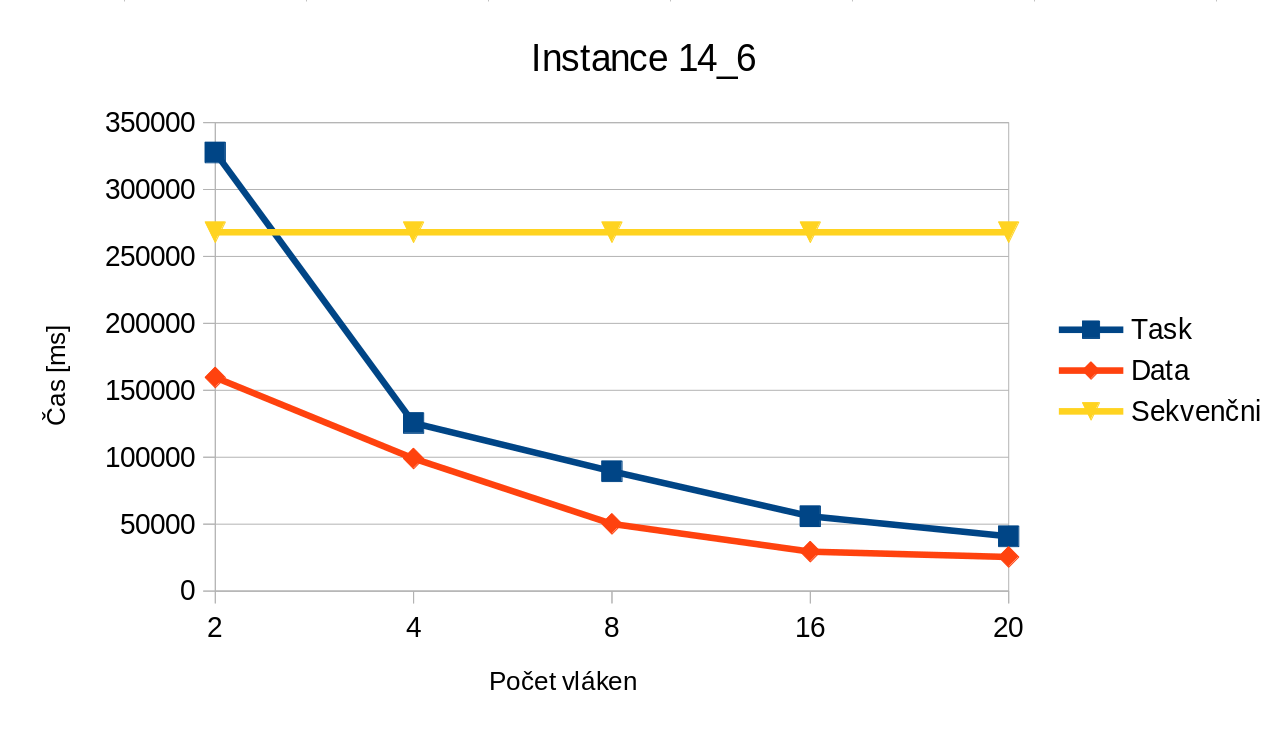
\includegraphics[width=1\linewidth]{images/12_6_2.png}%

    \caption{  Graf zobrazuje časovou závislost jednotlivých paralelních algoritmů a sekvenčního vzhledem k počtu přidělených vláken nad testovací instancí grafu 14\_6. Zajímavé je, že paralelní algoritmus využívající OpenMP Task paralelismus je se dvěmi vlákny dokonce pomalejší než sekvenční řešení. Toto chování vzhledem k relativně velkému overheadu bylo autorem předpokládáno. Jako velmi překvapující ale je, že se zvyšujícím počtem vláken se výkon Task paralelismu velmi přiblížil k datovému a při 20ti vláknech je rozdíl velmi malý (u instancí 15\_6 a 18\_5 ještě nižší). Autor předpokládal znatelně větší rozdíl ve prospěch datového paralelismu.}%
    \label{fig:126}
\end{figure}


\begin{figure}[H]%
    \centering%
    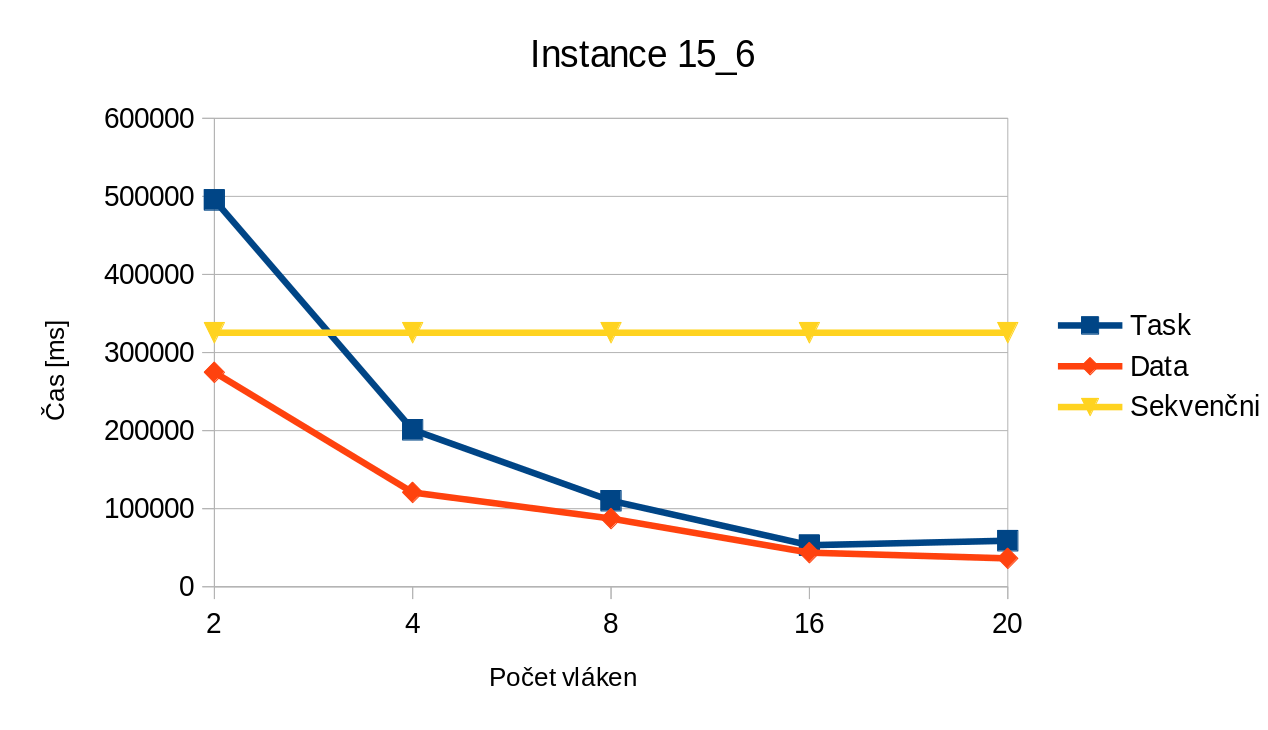
\includegraphics[width=1\linewidth]{images/15_6.png}%

    \caption{ Graf zobrazuje časovou závislost jednotlivých paralelních algoritmů a sekvenčního vzhledem k počtu přidělených vláken nad testovací instancí grafu 15\_6. Oproti grafu 14\_6  Graf \ref{fig:126} je zde možné pozorovat superlineární zrychlení kromě task, tak i u datové paralelismu mezi využití 2 a 4 vláken (274~s vs. 120~s). }%
    \label{fig:156}
\end{figure}

\begin{figure}[H]%
    \centering%
    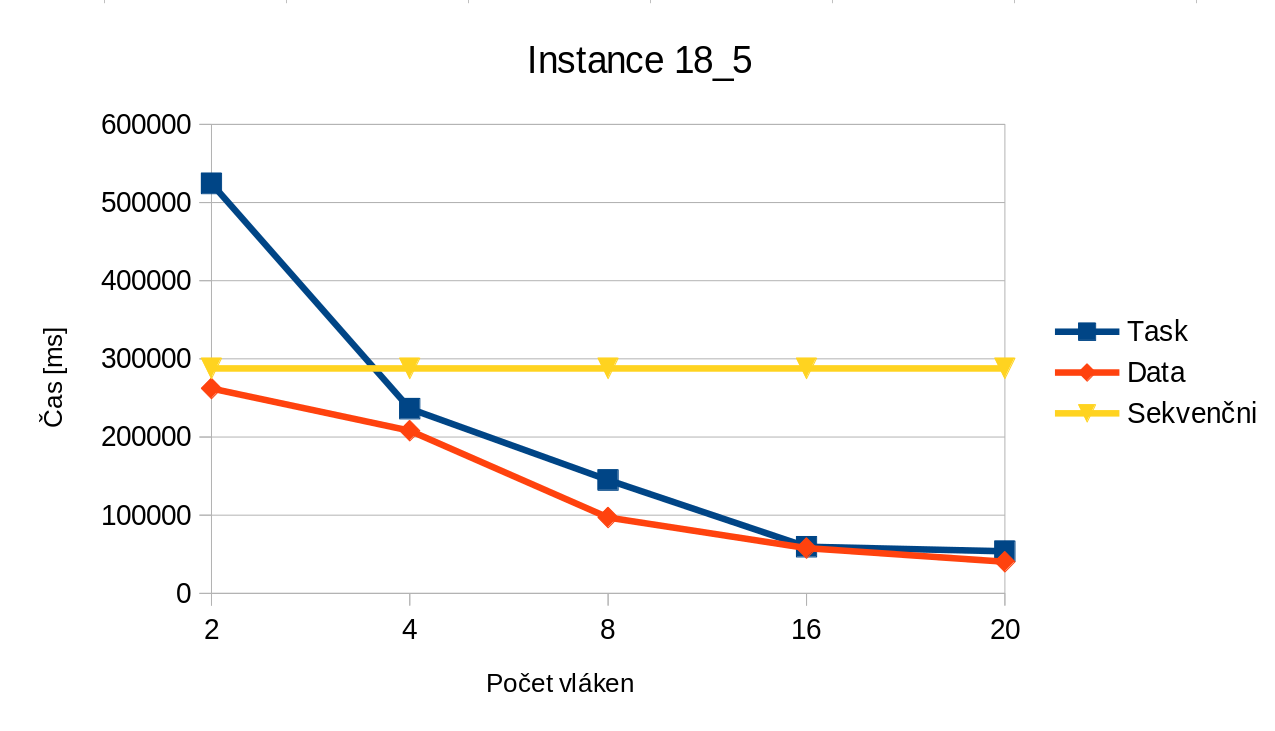
\includegraphics[width=1\linewidth]{images/18_5_2.png}%
    \caption{Graf zobrazuje časovou závislost jednotlivých paralelních algoritmů a sekvenčního vzhledem k počtu přidělených vláken nad testovací instancí grafu 18\_5. Podobné chování algoritmů viz. komentář u grafu s instancí 14\_6  Graf \ref{fig:126}.  }%
    \label{fig:185}
\end{figure}

\subsection{Vizualizace a interpretace OpenMP - zrychlení}

% ------ -- - - - - - -- -- -- - - - -- - - -- - - - - - -- - %
\begin{figure}[H]%
    \centering%
    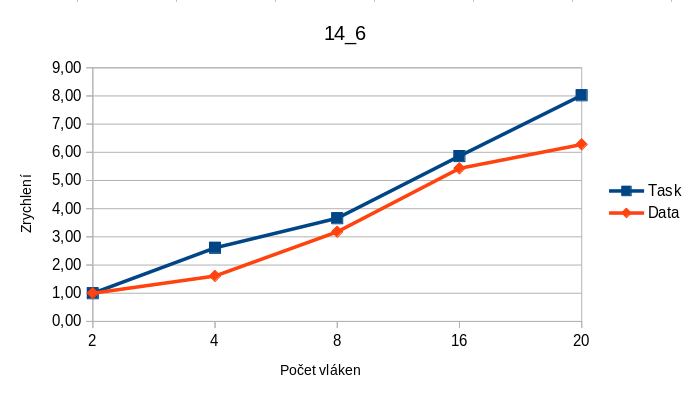
\includegraphics[width=1\linewidth]{images/acc_14_6.png}%

    \caption{Graf zobrazuje zrychlení vzhledem k početu vláken. Je zde možné pozorovat superlineární zrychlení pro task paralelismus při využití 4 vláken (2,61) - toho je možné dosáhnout díky implementovanému ořezávání, kdy je paralelně nalezeno řešení o doposud nejvyšší ceně a protože je tato hodnota sdílena mezi vlákny, tak ostatní mohou ihned zahodit rozpracovaná řešení, která této hodnoty nemohou dosáhnout (zjištěno na základně horního odhadu). Je zde také dobře viditelná lineární škálovatelnost u obou algoritmů. }%
    \label{fig:acc126}
\end{figure}


\begin{figure}[H]%
    \centering%
    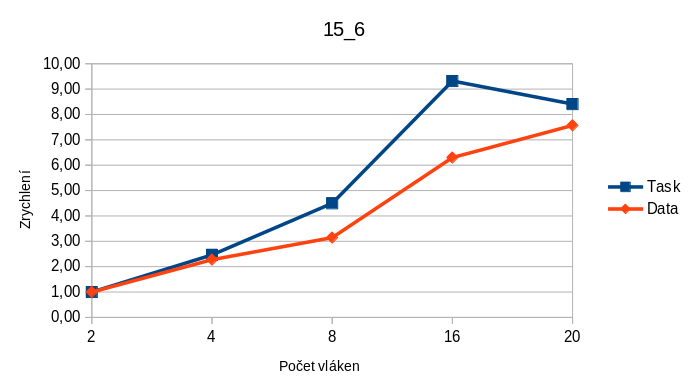
\includegraphics[width=1\linewidth]{images/acc_15_6.png}%

    \caption{Graf zobrazuje zrychlení vzhledem k početu vláken. Oproti předchozímu Grafu \ref{fig:acc126} je zde možné pozorovat superlineární zrychlení kromě task i u datové paralelismu při využití 4 vláken (2,28). Task paralelismus zde dosahuje superlineárního zrychlení v téměř všech měřených případech, pouze při 20 vláknech ne.}%
    \label{fig:acc156}
\end{figure}

\begin{figure}[H]%
    \centering%
    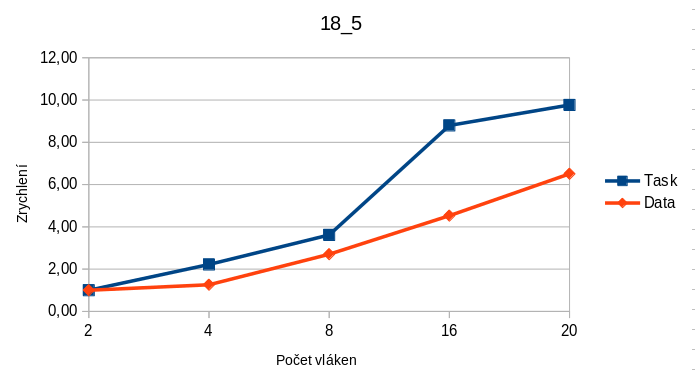
\includegraphics[width=1\linewidth]{images/acc_18_5.png}%
    \caption{Graf zobrazuje zrychlení vzhledem k početu vláken. Dochází zde opět k superlineárnímu škálování u task paralelismu.  }%
    \label{fig:acc185}
\end{figure}

\begin{table}[ht]%
    \begin{center}%
        \begin{tabular}{r|ccccc}%
            2 vlákna  & sekvenční & task & datový \\
            \hline%
            14\_6     & 1         & 0,82 & 1,68   \\
            15\_6     & 1         & 0,66 & 1,18   \\
            18\_5     & 1         & 0,55 & 1,10   \\
            \hline%
            4 vlákna  & sekvenční & task & datový \\
            \hline%
            14\_6     & 1         & 2,14 & 2,71   \\
            15\_6     & 1         & 1,62 & 2,70   \\
            18\_5     & 1         & 1,22 & 1,38   \\
            \hline%
            8 vláken  & sekvenční & task & datový \\
            \hline%
            14\_6     & 1         & 3,00 & 5,34   \\
            15\_6     & 1         & 2,95 & 3,73   \\
            18\_5     & 1         & 1,99 & 2,97   \\
            \hline%
            16 vláken & sekvenční & task & datový \\
            \hline%
            14\_6     & 1         & 4,80 & 9,12   \\
            15\_6     & 1         & 6,12 & 7,46   \\
            18\_5     & 1         & 4,83 & 4,98   \\
            \hline%
            20 vláken & sekvenční & task & datový \\
            \hline%
            14\_6     & 1         & 6,56 & 10,55  \\
            15\_6     & 1         & 5,52 & 8,97   \\
            18\_5     & 1         & 5,36 & 7,15   \\
        \end{tabular}%
        \caption{Obsahuje vypočtené zrychlení algoritmů vůči sekvenčnímu řešení - vypočteno jako poměr sekvenčního času a daného algoritmu pro 3 testovací instance a různý počet vláken. Paralelní algoritmy dle měření škálují téměř lineárně, což je velmi dobrý výsledek. K superlineárnímu zrychlení task paralelismu došlo nad všemi měřenými instancemi při využití dvou a čtyř vláken viz. Graf \ref{fig:126}, Graf \ref{fig:156}, Graf \ref{fig:185}, u datového pouze v případě instance 15\_6 viz. Graf \ref{fig:156}. Dle výsledků se datový paralelismus ukázal jako naprosto dominantní nad task paralelismem, ve všech testovaných případech.}%
    \end{center}%
\end{table}

\subsection{Měření MPI}
V průběhu měření MPI autor narazil na vzláštní chování při měření běhu implementace na školním clusteru. Prvnostní testování nad malými instancemi \~ doba výpočtu pár vteřina byla bez problémů. Při spuštění nad většími instancemi s výpočtem v řádu minut začalo docházet k náhodnému ``zaseknutí`` výpočtu. Master i Slave se korektně spustily, Master vygeneroval úkolů a odeslal první k řešení na Slave. Zde docházelo k nějakému typu zaseknutí, kdy Slave již nikdy neodeslal žádný výsledek. Toto byl časově závislý problém \~ někdy nastal ihned, někdy Slave odeslal desítky řešení a až potom došlo k zaseknutí. Testováno se 2 a 3 Slave procesy. Nikdy nedošlo k žádné MPI chybě - vzhledem k implementaci, autorovi se jako nejpravděpodobnější jeví možný problém v použité knihovně Boost nebo využití OpenMP kritické sekce k paralelní obsluze MPI volání (i přes to, že bylo MPI příslušně iniciováno). Implementace byla následně otestována na autorově stanici se systémem Ubuntu s novější verzí MPI a OpenMP z repozitářů a daný problém nikdy nenstal i při běhu desítek minut. K rozsáhlejšímu testování na školním clusteru autor nakonec nemohl přistoupil, z důvodu vysokého vytížení clusteru (přes 600 úloh čekající na spuštění ve frontě). Testování MPI bylo tedy nakonec naměřeno na stroji s následující konfigurací: CPU Ryzen 3600 (6 jader/12 vláken), RAM 24 GB, OS Fedora 35. Implementace byla při měření spouštěna v Docker kontejneru s obrazem Ubuntu 20.04. Vzhledem k tomu, že daný stroj má pouze jeden procesor, tak bude měření zaměřeno na spuštění více procesů s menším počtem vláken. Měření s jedním procesem nebylo provedeno, protože při architektuře Master-Slave je potřeba alespoň 2 procesy, aby jeden rozděloval práci a druhý prováděl výpočty.


\begin{figure}[H]%
    \centering%
    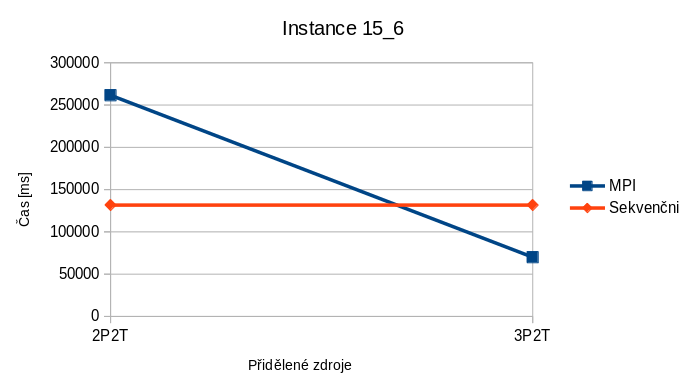
\includegraphics[width=1\linewidth]{images/mpi_15_6.png}%
    \caption{Graf zobrazuje časovou závislost sekvenčního a paralelního MPI algoritmu vzhledem k přiděleným prostředkům - 2 procesy/2 vlákna, 3 procesy/ 2 vlákna, měřeno na autorově stanici. MPI algoritmus s jedním výpočetním procesem je 2krát pomalejší než sekvenční řešení. To je způsobeno pravděpodobně samotným MPI prostředím, protože spustit jednotlivé procesy a připrava komunikace trvá dlouhou dobu. Toto měření nelze moc dobře porovnávat s předešlím, které bylo měřeno na clusteru, kde procesory jsou jinak výkonné. Je zde ale vidět superlineární zrychlení mezi využitím 2 a 3 procesů (261~s vs. 70~s). Graf pro instanci 14\_6 vypadá obdobně.}%
\end{figure}

\begin{figure}[H]%
    \centering%
    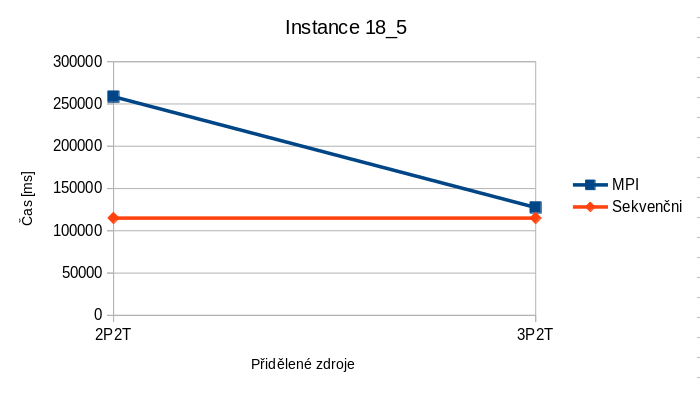
\includegraphics[width=1\linewidth]{images/mpi_18_5.png}%
    \caption{Graf zobrazuje časovou závislost sekvenčního a paralelního MPI algoritmu vzhledem k přiděleným prostředkům - 2 procesy (Master, Slave) / 2 vlákna, 3 procesy (Master, Slave, Slave) / 2 vlákna, měřeno na autorově stanici. Zde je možno pozorovat vzláštní jev. Zatímco u instancí 14\_6 a 15\_6 došlo ke znatelnému zrychlení při dvou výpočetních procesech, tak u této instance jsou i dva výpočetní procesy pomalejší než-li sekvenční algoritmus. Autor toto chování přisuzuje částečně dlouhému spuštění MPI prostředí a především potom ke specifičnosti této instance vůču způsobu generování úkolů (jak pro MPI procesy, tak následně pro datový paralelismus). Dochází zde k souhře těchto dvou okolností, které zvyšující neefektivitu ořezávání procházeného prostoru - hodnotné řešení je nalezeno mnohem později než při sekvenčním řešení a ořezávání nemůže být efektivní. Možné řešení s lepšími statistickými vlastnostmi by mohlo vést přes náhodné permutování vygenerované posloupnosti úkolů k řešení. Pro lepší představu by ale bylo potřeba se nejprve podívat na efektivitu pro větší množství instancí.}%
\end{figure}

\section{Zhodnocení a závěr}
Cílem této práce byla implementace a analýza paralelních algoritmů s využitím OpenMP a MPI. Nejprve byla vytvořena implementace sekvenčního řešení v jazyce C++, jako výchozí bod. Následně byly implementovány 3 paralelní algoritmy: task paralelismus (OpenMP), datový paralelismus (OpenMP), kombinace MPI a OpenMP datového paralelismu. Následně byla změřena časová závislost na počtu přiřazených prostředků nad třemi zvolenými testovacími instancemi. Task paralelismus dosáhl překvapivě dobré škálovatelnosti (oproti autorově očekávání), pouze pro dvě vlákna převládl vyšší overhead jinak škáluje často lépe jak lineárně. Datový paralelismus se ukázal jako dominantní výkonově ve všech měřených případech a dosáhl lineárního škálování. Při měření se prokázalo superlineární škálování u všech paralelních algoritmů alespoň v jednom případě, které je způsobeno implementovaným ořezáváním prostoru, kdy si vlákna a procesy sdílí hodnotu, na základě které se provádí ořez.

MPI algoritmus se autorovi nepodařilo otestovat na školím clusteru, z důvodu zamrzání výpočtu z přičiny, kterou se bohužel nepodařilo indentifikovat. Měření tedy bylo provedeno na autorově stanici. U měření lze porozovat poměrně velký overhead, které má samotné MPI a je tedy vidět, že využití se vyplatí až pro dostatečně velké instance. Také je zde vidět superlineární zrychlení u jedné instance.

Až na problém s MPI je autor s výsledkem práce spokojený. Algoritmy se ukázaly nad měřenými daty přibližně lineárně škálovatelné a v některých případech i superlineárně.


\newpage

\begin{table}[]
    \begin{tabular}{l|lllll}
        14\_6     & 2          & 4          & 8          & 16         & 20         \\ \hline
        Task      & 327 639,67 & 125 485,67 & 89 482,00  & 55 847,33  & 40 831,33  \\
        Data      & 159 536,00 & 99 033,00  & 50 177,33  & 29 385,00  & 25 413,67  \\
        Sekvenčni & 268 056,60 & 268 056,60 & 268 056,60 & 268 056,60 & 268 056,60 \\ \hline
        15\_6     & 2          & 4          & 8          & 16         & 20         \\ \hline
        Task      & 495 475,33 & 200 969,67 & 110 131,00 & 53 166,33  & 58 914,00  \\
        Data      & 274 598,00 & 120 690,33 & 87 294,33  & 43 586,67  & 36 269,67  \\
        Sekvenčni & 325 316,00 & 325 316,00 & 325 316,00 & 325 316,00 & 325 316,00 \\ \hline
        18\_5     & 2          & 4          & 8          & 16         & 20         \\ \hline
        Task      & 524 318,67 & 236 173,67 & 144 919,67 & 59 601,67  & 53 677,00  \\
        Data      & 262 002,67 & 208 052,00 & 96 892,67  & 57 845,00  & 40 256,00  \\
        Sekvenčni & 287 655,00 & 287 655,00 & 287 655,00 & 287 655,00 & 287 655,00
    \end{tabular}
    \caption{Tabulka obsahuje průměrné naměřené časy (v ms) pro různé algoritmy s různým počtem vláken a nad různými instancemi.}
\end{table}

\begin{table}[]
    \begin{tabular}{l|lllll}
        14\_6 & 2    & 4    & 8    & 16   & 20   \\ \hline
        Task  & 1,00 & 2,61 & 3,66 & 5,87 & 8,02 \\
        Data  & 1,00 & 1,61 & 3,18 & 5,43 & 6,28 \\ \hline
        15\_6 & 2    & 4    & 8    & 16   & 20   \\ \hline
        Task  & 1,00 & 2,47 & 4,50 & 9,32 & 8,41 \\
        Data  & 1,00 & 2,28 & 3,15 & 6,30 & 7,57 \\ \hline
        15\_5 & 2    & 4    & 8    & 16   & 20   \\ \hline
        Task  & 1,00 & 2,22 & 3,62 & 8,80 & 9,77 \\
        Data  & 1,00 & 1,26 & 2,70 & 4,53 & 6,51
    \end{tabular}
    \caption{Tabulka obsahuje vypočtené zrychlení pro různé instance.}
\end{table}
\end{document}